\section{Metodologia}
    \subsection{Material Utilizado}
        \begin{itemize}
    \item [1] Bobina de Helmholtz 
        \begin{itemize}
             \item [n] 140 espiras
             \item [D] 22,3cm
             \item [d] 20,2cm
             \item [l] 1,13cm
             \item [L] 10,26cm
        \end{itemize}
    \item [1] Bússola
    \item [1] Ímã permanente cilíndrico 
        \begin{itemize}
             \item [D] 0,6cm
             \item [l] 2,53cm
             \item [m] 5,1616g
        \end{itemize}
    \item [1] Multímetro
    \item [1] Resistor de potência
    \item [1] Fonte de alimentação
    \item [1] Cronômetro
    \item [6] Fios de ligação
\end{itemize}

    \subsection{Especificações do Multímetro digital MD-6680}
        Para a medição das tensões, 
        coloca-se a chave seletora para a posição de tensão 
        e pressiona-se o botão \textbf{DC} conectando duas das pontas
        de prova nos terminais \textbf{V} e \textbf{COM} e as outras em 
        paralelo com o dispositivo a ser medido.
        \paragraph{Obs.:} Resistência interna do voltímetro: $R_{v_{int}} = 10^6 \Omega$ 
        \paragraph{Obs.:} Resolução da escala utilizada: $\Delta V = 10^{-2} V$ 

    \subsection{Procedimento}
        \subsubsection{Montagem do Experimento}
            \paragraph{Para a realização do experimento em placas paralelas}
            Em uma cuba plástica foi colocada uma placa milimetrada 
            e a solução de sulfato de cobre. Em seguida, foram 
            colocadas as duas placas de cobre paralelamente a 
            uma distância de \textbf{d = 180mm}. 
            A fonte de tensão foi conectada às duas placas, 
            e o multímetro foi conectado à placa que era o 
            terminal negativo da fonte e ao cabo ponta de prova 
            onde variamos os locais para a medição.
            \paragraph{Para a realização do experimento com a ponta}
            Foi repetido a montagem usada para as placas paralelas, adicionando a ponta de cobre à placa que era o terminal positivo da fonte
            \paragraph{Para a realização do experimento com o aro}
            Foi repetido a montagem usada para as placas paralelas, 
            adicionando o aro de cobre no relativo centro da cuba. 
            Sendo primeiro testado com o aro sem conexão com as 
            placas eletrizadas, em seguida foi conectado o aro à 
            placa que era o terminal positivo da fonte, 
            usando um cabo com grampo.
            \newline
            \newline
            Usou-se uma tensão de \textbf{2V} 
            para o experimento, utilizando a Fonte de Tensão, 
            e o multímetro na posição de tensão para encontrar os 
            pontos na solução com o mesmo potencial elétrico. 
        \subsubsection{Determinando equipotenciais}
            Utilizando a ponta de prova, foram determinados
            "pontos iniciais", com a ajuda da placa milimetrada. 
            Tais pontos possuíam uma diferença de potencial 
            $\Delta V$ devido à solução de sulfato de cobre 
            funcionar como uma resistência. A cada 20 mm foram
            encontrados os pontos com a mesma diferença de 
            potencial $\Delta V$ que o ponto inicial, os mesmo 
            então foram marcados em sua respectiva posição em 
            uma folha milimetrada. Os pontos foram ligados, 
            formando linhas chamadas de equipotenciais, 
            devido ao fato de possuírem a mesma diferença 
            de potencial em seu percurso.
            \newline
            \newline
            Em especial, no experimento com aro, medimos a 
            diferença de potencial $\Delta V$ de alguns pontos no 
            interior do aro, para tentarmos identificar o 
            comportamento do campo elétrico dentro de uma 
            Gaiola de Faraday.
        \subsubsection{Encontrando o vetor e o módulo do campo elétrico empiricamente}
            Também foi possível encontrar o vetor e o modulo
            do campo elétrico de maneira empírica. Dado que: 
            $$\bar{E} = - \nabla V$$
            podemos encontrar o campo elétrico medindo o gradiente
            do campo, ao invés de medir as equipotenciais
            e calcular seu gradiente.
            \newline
            \newline
            Desta maneira, ao invés de conectar um terminal
            do multímetro à placa e a outra na ponta de prova,
            conectamos os terminais a duas pontas de provas 
            e as unimos com uma fita adesiva, tornando-os 
            dois terminais de distância fixa.
            \newline
            \newline
            Escolhendo um ponto de partida, mantemos uma 
            ponta de prova fixa, rotacionando a outra ponta, 
            até encontrar a maior variação de potencial. 
            \newline
            \begin{figure} [ht]
                \centering
                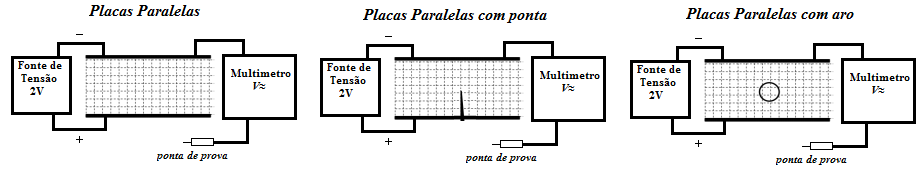
\includegraphics[width=1.0\textwidth]{modelos}
                \caption{Modelos utilizados}
                \label{fig:modelos}
            \end{figure}
            \newline
            Assim, teremos o vetor do gradiente e o módulo 
            do mesmo em pequenas distâncias d entre as pontas 
            de prova. Fazendo uma "derivada empírica".